\documentclass{rapport_stage}

% package ajouté au dessus de la template

\usepackage{xcolor}
\usepackage{csquotes}
\usepackage{bookmark}
\usepackage{enumitem}
\usepackage{pifont}
\usepackage[style=ieee,backref=true]{biblatex}



% Lien vers la bibliographie

\bibliography{bibliography_rapport_de_stage}

% Variable utilisé par la template

\def\reportTitle{Analyse et Conception d'Eledone : un outil de déploiement de simulations pour l'utilisateur profane} % Titre du rapport de stage

\def\reportAuthor{Théo Piacentini}
\def\reportAuthorEmail{\email{theo.piacentini@gmail.com}} % Courriel de l'élève

\def\reportSupervisor{Jean-François Santucci, Laurent Capocchi} % Nom des tuteurs

\def\reportCompany{UMR 6134 CNRS} % Nom de l'entreprise d'accueil

% % ====================== Début Document  ==========================



\begin{document}

\maketitle
\pagenumbering{roman}

\cleardoublepage

Théo Piacentini \\
Résidence Le Boticelli \\
20620 Biguglia \\
+33 (0)7 77 78 55 54 \\
\href{mailto:theo.piacentini@gmail.com}{\nolinkurl{theo.piacentini@gmail.com}}

\smallskip

Jean-François Santucci \\
Professeur Titulaire \\
Université de Corse "Pasquale Paoli"\\
UMR CNRS 6134\\
Quartier Grossetti\\
BP 52, 20250 Corte\\
tel : +33 4 95 45 02 30\\
\href{mailto:santucci-j@univ-corse.fr}{\nolinkurl{santucci-j@univ-corse.fr}}

\smallskip

Laurent Capocchi \\
Maitre de Conférence en Informatique \\
Université de Corse "Pasquale Paoli"\\
UMR CNRS 6134\\
Quartier Grossetti\\
BP 52, 20250 Corte\\
tel : +33 4 95 45 02 30\\
\href{mailto:capocchi@univ-corse.fr}{\nolinkurl{capocchi@univ-corse.fr}}

\cleardoublepage
\phantomsection
\section*{Remerciements}
\addcontentsline{toc}{chapter}{Remerciements}

{\color{green}
  À compléter à la fin
}

\clearpage
\phantomsection

\renewcommand{\baselinestretch}{0.5}\normalsize
\tableofcontents
\renewcommand{\baselinestretch}{1.0}\normalsize
\cleardoublepage

\pagenumbering{arabic}
\setcounter{page}{1}

\newglossaryentry{pfonctionnel}{
  name=paradigme fonctionnel,
  description={
      à définir
    }
}

\newglossaryentry{pdonnées}{
  name=paradigme orienté données,
  description={
      à définir
    }
}


\chapter*{Introduction}  % no number
\addcontentsline{toc}{chapter}{Introduction} % add it to the ToC

Cette année de licence 3 m'a beaucoup appris et convaincu que j'avais trouvé ma voie en me
permettant de me faire une culture informatique tout en participant à des projets proches du réel.
J'ai pu au cours de celle-ci définitivement me tourner vers la recherche en gardant cependant un
gout pour le développement. C'est donc dans l'optique de lier tout cela que j'ai choisis ce stage
avec l'idée de travailler sur un projet de développement lié à la recherche.

\section*{Pourquoi choisir ce stage ?}

J'ai toujours été intéressé par la recherche, je voulais donc découvrir ce
métier dans le cadre de mon stage. Les cours que j'ai eues avec M. Santucci en
1\iere \ et 3\ieme \ année de licence m'ont beaucoup plus, car ils étudiaient des domaines à mon
avis sous-explorés de l'informatique, car souvent considérer comme trop formels
comme le \gls{pfonctionnel}
\footnote{Je parle ici de l'"original", celui basé sur un formalisme mathématique que l'on peut
  retrouver dans le LISP ou de nos jours, sous une certaine forme, dans des langages comme Haskell.}
et le \gls{pdonnées}. C'est dans l'optique de lier ce formalisme à des projets projet de
développement que j'ai voulue effectuer ce stage avec lui.\\

L'une des autres raisons est ma volonté d'étudier le domaine de la modélisation et de la
simulation qui ne sont pas explorés durant cette année de licence. Cela
m'aidera à compléter mon parcours d'étude de l'informatique tout en me permettant
d'explorer un domaine proche des mathématiques, un autre de mes centres d'intérêts. \\

Enfin l'idée de poursuivre une thèse après mon master à l'Université de Corse
me plait beaucoup et un stage dans la recherche est une étape nécessaire à
cela en plus de me permettre de savoir si cet objectif est viable pour moi.

\section*{Les objectifs}

\begin{itemize}[label=$\bullet$]
  \item Le but pour moi est d'avoir une première expérience dans la rechercher et dans l'informatique professionnel
  \item L'idée est de trouver des sujets à approfondir pour l'année prochaine
\end{itemize}

Comme vu précédemment le but principal de ce stage pour moi est d'explorés le monde de la recherche
l'écriture de ce rapport est donc un bon moyen de tester la création de document proche de papiers
scientifiques, ainsi il fut produit avec l'aide d'outils professionnels destiné à la recherche
tel que Zotero pour les sources et LaTeX pour l'écriture et la création du document \\

L'autre but de ce projet est l'application en condition réelle du formalisme UML vu cette année.
L'idée est, en effet, de créer une application en respectant un modèle d'Analyse, Conception,
Réalisation et Évaluation tout en sachant se détacher de tout cela se je le juge nécessaire dans
l'optique d'apprendre le plus possible tout en développant un logiciel de qualité. \\

Pour finir le but est aussi de trouver des pistes d'exploration dans des sujets qui m'intéressent
pour mon master l'année prochaine. En effet, je compte poursuivre mes études à Corte pour apprendre
le développement web et mobile, mais espère bien pouvoir lier cela à la recherche dans mes projets
tout au long de mon parcours.

\cleardoublepage

% ====================== PARTIE 1  ==========================




\part{Présentation du stage}

\chapter{Présentation de l'Organisme}

\section*{Laboratoire Sciences Pour l'Environnement de l'Université de Corse (UMR CNRS 6134 SPE)}

\begin{figure}[ht]
  \centering
  
\includegraphics[width=15cm]{figures/logo_SPE.png}
  \caption{Logo du laboratoire SPE de l'Université de Corse}
  \label{fig:logo-SPE}
\end{figure}


Le laboratoire Sciences Pour l'Environnement (UMR 6134 SPE) est une Unité Mixte de Recherche
rattachée à l'Université de Corse, à l'Institut des Sciences de l'Ingénierie et des Systèmes et à
l'Institut Écologie et Environnement du CNRS. C'est une unité pluridisciplinaire dont le personnel
est rassemblé en six équipes thématiques, appelées "projets structurants"
\cite{santoni_presentation_2022} :

\begin{itemize}
  \item Projet EnR : Énergies Renouvelables
  \item Projet FEUX : Feux de forêts
  \item Projet RN : Ressources Naturelles
  \item Projet GEM : Gestion et valorisation des Eaux en Méditerranée
  \item Projet SISU : Simulation Informatique et Systèmes Ubiquitaires
  \item Projet COMPA : Champs, Ondes, Mathématiques et APplications
\end{itemize}

Les projets EnR, FEUX, RN et GEM sont en lien avec la transition écologique et les risques
environnementaux tandis que les projets SISU et COMPA développent des concepts et outils
en collaboration avec les autres équipes tout en développant des travaux de recherche dans leurs
domaines respectifs. \\

% penser à ajouter certains termes au glossaire

Le projet auquel participent mes deux maitres de stage M. Laurent Capocchi et M. Jean-François
Santucci, et donc celui dans lequel je fais mon stage, est le projet SISU dédier à la simulation
informatique et aux Systèmes Ubiquitaires il accueille la plupart des chercheurs en Informatique de
l'Université de Corse.

\begin{figure}[ht]
  \centering
  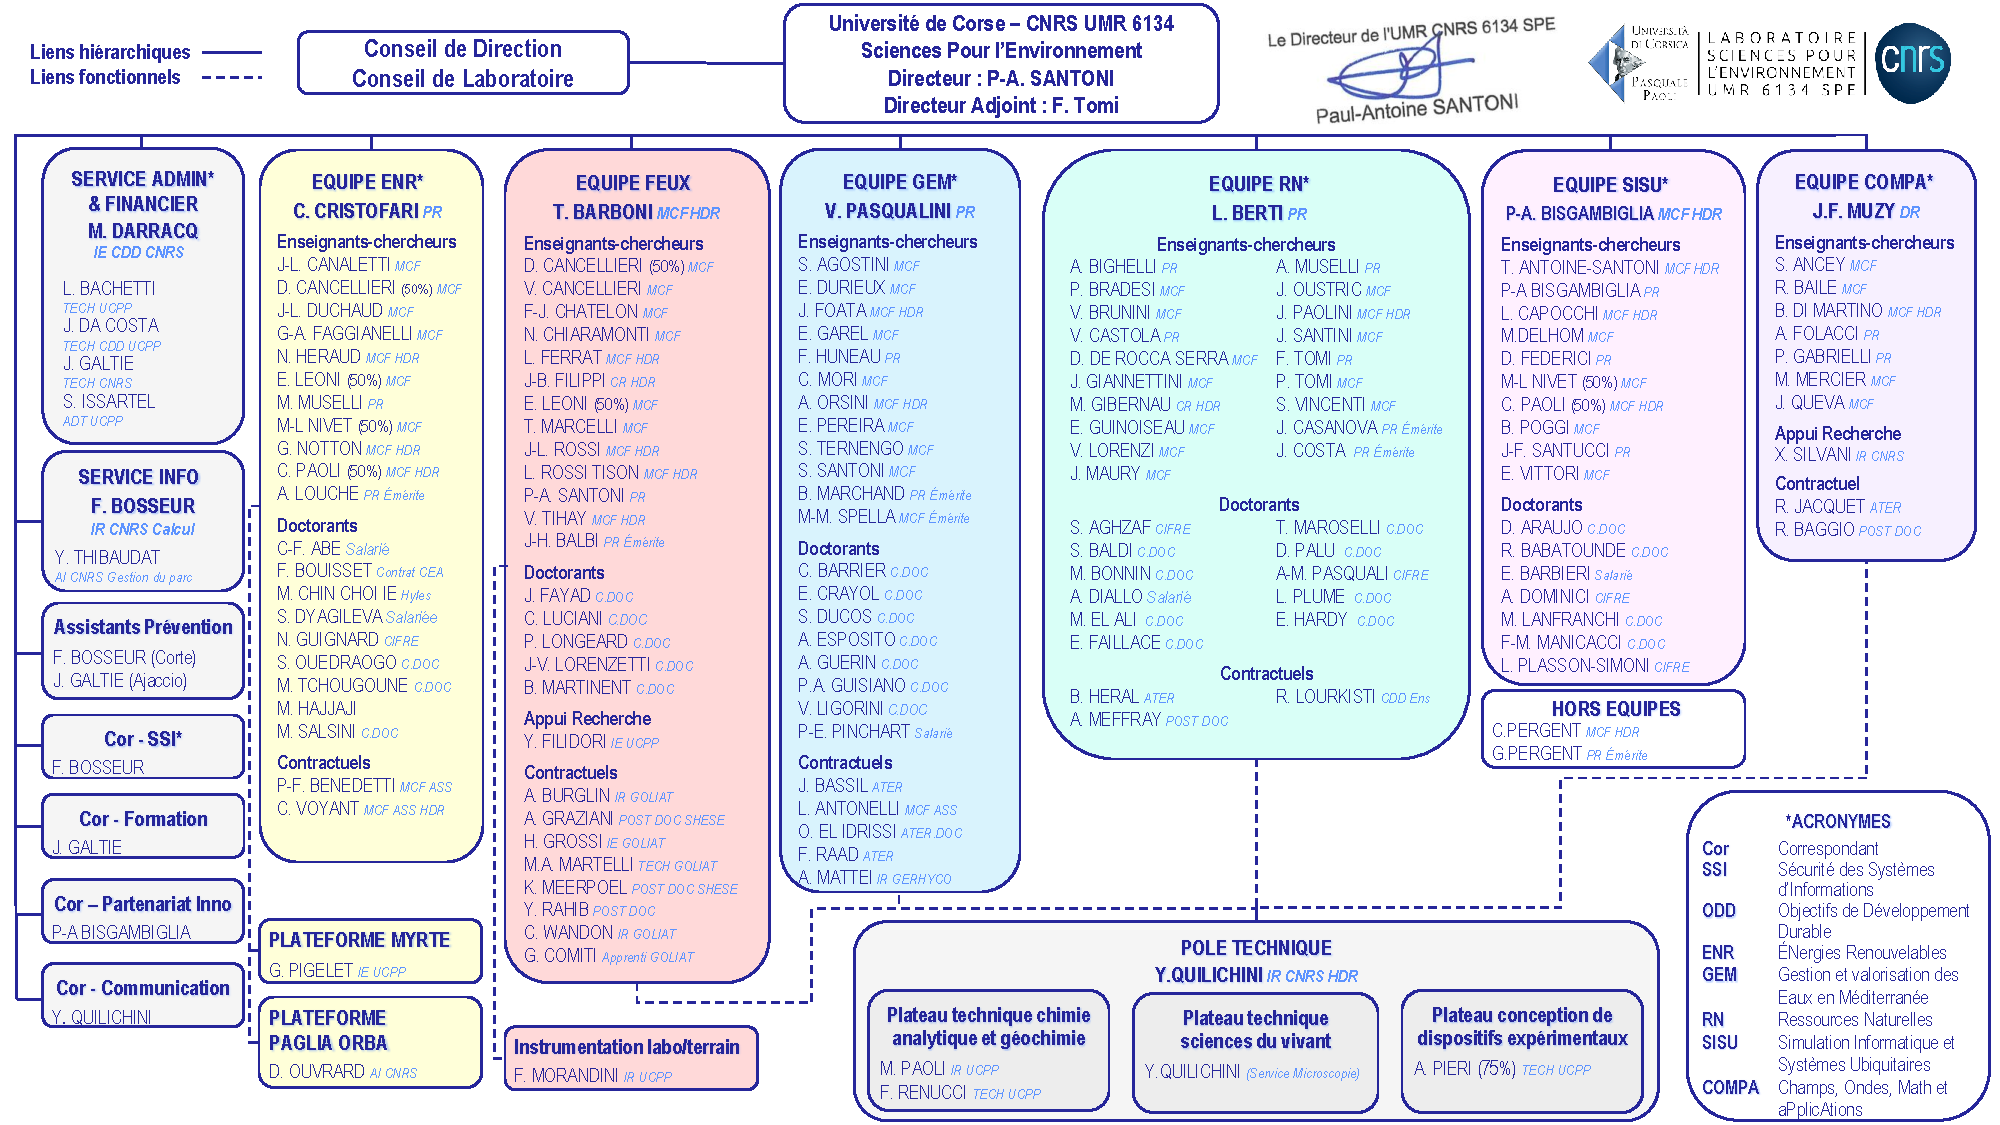
\includegraphics[width=15cm]{figures/Organigramme_UMR.pdf}
  \caption{Organigramme du laboratoire SPE de l'Université de Corse \cite{santoni_presentation_2022}}
  \label{fig:Organigramme-SPE}
\end{figure}


\section*{Le Projet SISU : Simulation Informatique et Systèmes Ubiquitaires}

\begin{itemize}[label=$\bullet$]
  \item Expliquer le projet SISU
  \item Trouver les différents sujet lié a SISU
\end{itemize}

Dirigé par M. Paul-Antoine Bisgambiglia, le projet SISU est constitué de deux approches :
L'aspect scientifique du projet qui est fondé sur la définition d'une approche générique de
Modélisation et Simulation de systèmes complexes tandis que l'aspect technologique concerne
la mise en œuvre des concepts et outils dans le cadre d'application concrète.

Dans ce projet le travail de M. Capocchi et M. Santucci concerne plutôt la première partie
auquel ils participent principalement par le biais de papiers lié au formalisme DEVS
\cite{capocchi_devs_2022} \cite{capocchi_towards_2023} et au développement d'un logiciel aidant à
la création de modèle de simulation : DevSimPy \cite{l_what_2023}. Le stage que j'ai effectué
s'est donc déroulé dans leur équipe et le projet que je vous présente avec ce rapport fait suite
à leur travail.

\cleardoublepage

\chapter{Présentation de la tâche effectuée}

 {\color{green}
  À compléter à la fin
 }

\section*{Semaine 1}

\begin{itemize}[label=$\bullet$]
  \item Choix du projet rdv à l'IUT de Corte
  \item création de maquettes
  \item création de schémas
  \item Lecture des papiers
  \item début de l'état de l'art
\end{itemize}

\section*{Semaine 2}

\begin{itemize}[label=$\bullet$]
  \item Visioconférence pour discuter de l'avancé du projet et des décisions lié à celui-ci
  \item Découverte et utilisation de LaTeX pour l'écriture du rapport
  \item création du plan du rapport / projet
  \item avancé état de l'art
  \item Création de schémas
  \item Recherche de ressources liées à la simulation et aux systèmes distribués
  \item liaison des outils de schémas et de ressources avec LaTeX
\end{itemize}

\section*{Semaine 3}

\begin{itemize}[label=$\bullet$]
  \item The first item of the list. Je suis tr
\end{itemize}

\section*{Semaine 4}

\begin{itemize}[label=$\bullet$]
  \item The first item of the list.
\end{itemize}

\chapter{Définition du projet et de ses objectifs}

\section{Les origines scientifiques}

\begin{itemize}[label=$\bullet$]
  \item Décrire les papiers de M. Santucci et M. Capocchi \cite{capocchi_devs_2022} \cite{capocchi_towards_2023}
  \item description succincte de DEVS
\end{itemize}

\section{Description du projet}

\begin{itemize}[label=$\bullet$]
  \item Le concept est de créer un CMS autour de la simulation
  \item à la vue de la durée de stage un se contentera de la phase d'analyse et de la conception du projet
  \item Le projet doit être une base la plus solide possible que ce soit du côté des sources scientifiques que dans la conception même du logiciel
\end{itemize}

\section{Les objectifs}

\begin{itemize}[label=$\bullet$]
  \item The first item of the list.
\end{itemize}

\section{Explication de notre approche}

\begin{itemize}[label=$\bullet$]
  \item Au vu des objectifs on va considérer que tout choix technologique rationnel est faisable
  \item On va tout découpler au maximum pour rendre le travail en équipe possible
  \item On va se baser sur le modèle Analyse etc. tiré de l'UML
  \item On utilisera l'UML quand cela aura un sens ce n'est pas un devoir d'UML
  \item sourcé la méthode d'Analyse par un livre théorique \cite*{lonchamp_analyse_2015}
\end{itemize}



\bookmarksetup{startatroot}

% ====================== FIN ==========================

\chapter*{Conclusion}  % no number
\addcontentsline{toc}{chapter}{Conclusion}

{ \color{green}
  À faire à la fin
}

\begin{itemize}[label=$\bullet$]
  \item The first item of the list.
\end{itemize}% add it to the ToC


\appendix



% ====================== PARTIE 2  ==========================



\part{Analyse}

\begin{itemize}[label=$\bullet$]
  \item The first item of the list.
\end{itemize}

\newglossaryentry{cmsg}{name={CMS},
  description={definition des CMS}}

%%% define the acronym and use the see= option
\newglossaryentry{cms}{type=\acronymtype, name={CMS}, description={Content Management System}, first={CMS (Content Management System)\glsadd{cmsg}}, see=[Glossary:]{cmsg}}

\chapter{État de l'art}


\begin{itemize}[label=$\bullet$]
  \item Introduction de l'état de l'art (pourquoi ?, comment ?)
\end{itemize}

Le but de cette phase est de présenter "état des connaissances dans un domaine
donné. Au vu du caractère pluridisciplinaire de notre projet, il convient donc
de présenter succinctement les domaines sur lesquelles se base notre projet.
Nous en avons identifié trois : La modélisation et la simulation, les
\gls{cms}

\section{Modélisation et Simulation}

\begin{itemize}[label=$\bullet$]
  \item Parler de la place du domaine dans l'informatique et les sciences en général
\end{itemize}

\subsection*{Définition du domaine}

\begin{itemize}[label=$\bullet$]
  \item Présenter le domaine dans son ensemble \cite{oren_body_2023}
\end{itemize}

\newpage

\subsection*{Histoire du domaine}

\begin{itemize}[label=$\bullet$]
  \item Trouver une bonne source pour faire l'historique
\end{itemize}

\newglossaryentry{devsg}{name={DEVS},
  description={An Application Programming Interface (API) is a particular set
      of rules and specifications that a software program can follow to access and
      make use of the services and resources provided by another particular software
      program that implements that API}}

%%% define the acronym and use the see= option
\newglossaryentry{devs}{type=\acronymtype, name={DEVS}, description={Application
      Programming Interface}, first={DEVS (Discrete Event System Specification)\glsadd{devsg}}, see=[Glossary:]{devsg}}

\subsection*{\gls{devs}: Une approche formelle de la Simulation }

\begin{itemize}[label=$\bullet$]
  \item Utiliser le livre de Ziegler pour définir DEVS \cite{zeigler_theory_2019}
\end{itemize}

\subsection*{Les autres points de vue}

\begin{itemize}[label=$\bullet$]
  \item Présenter l'utilisation de la simulation dans des contextes moins formels dans d'autres sciences pour faire le lien
\end{itemize}

\section{Systèmes de gestion de contenu}


\subsection*{Définition des \gls{cms}}

\begin{itemize}[label=$\bullet$]
  \item Petite histoire des CMS
  \item donner la proportion des sites web créer à partir de CMS
  \item difficile d'avoir une vue d'ensemble non biaisé, mais certaines ressources feront l'affaire \cite{barker_web_2016}
\end{itemize}

\subsection*{Les outils proches de notre concept}

\begin{itemize}[label=$\bullet$]
  \item Parler des CMS qui créent des applications web
  \item Parler d'Anvil \cite{anvil_team_overview_nodate}
  \item Parler de Streamlit \cite{streamlit_team_streamlit_nodate}
  \item Parler d'Amazon Honeycode. \cite{honeycode_team_no-code_nodate}
\end{itemize}

\section{Les systèmes distribués}

\begin{itemize}
  \item Parler des paradigmes liés en se basant sur des livres scientifiques \cite*{tanenbaum_distributed_2007} \cite*{coulouris_distributed_2012}
  \item Parler ensuite de l'approche plus récente à l'aide des conteneurs et des gestionnaires \cite*{burns_designing_2018} \cite*{kleppmann_designing_2017}
\end{itemize}

\chapter{Analyse globale}

\begin{itemize}[label=$\bullet$]
  \item Reprendre les papiers de M. Santucci et M. Capocchi \cite*{capocchi_devs_2022} \cite*{capocchi_towards_2023}
  \item Présenter à partir de là le fonctionnement global attendu de l'application
  \item s'aider de plusieurs schémas avec légende pour expliquer le concept
\end{itemize}

{ \color{green}
exemple de schéma réalisé à l'aide de Draw.io (à améliorer)
}

\begin{figure}[ht]
  \centering
  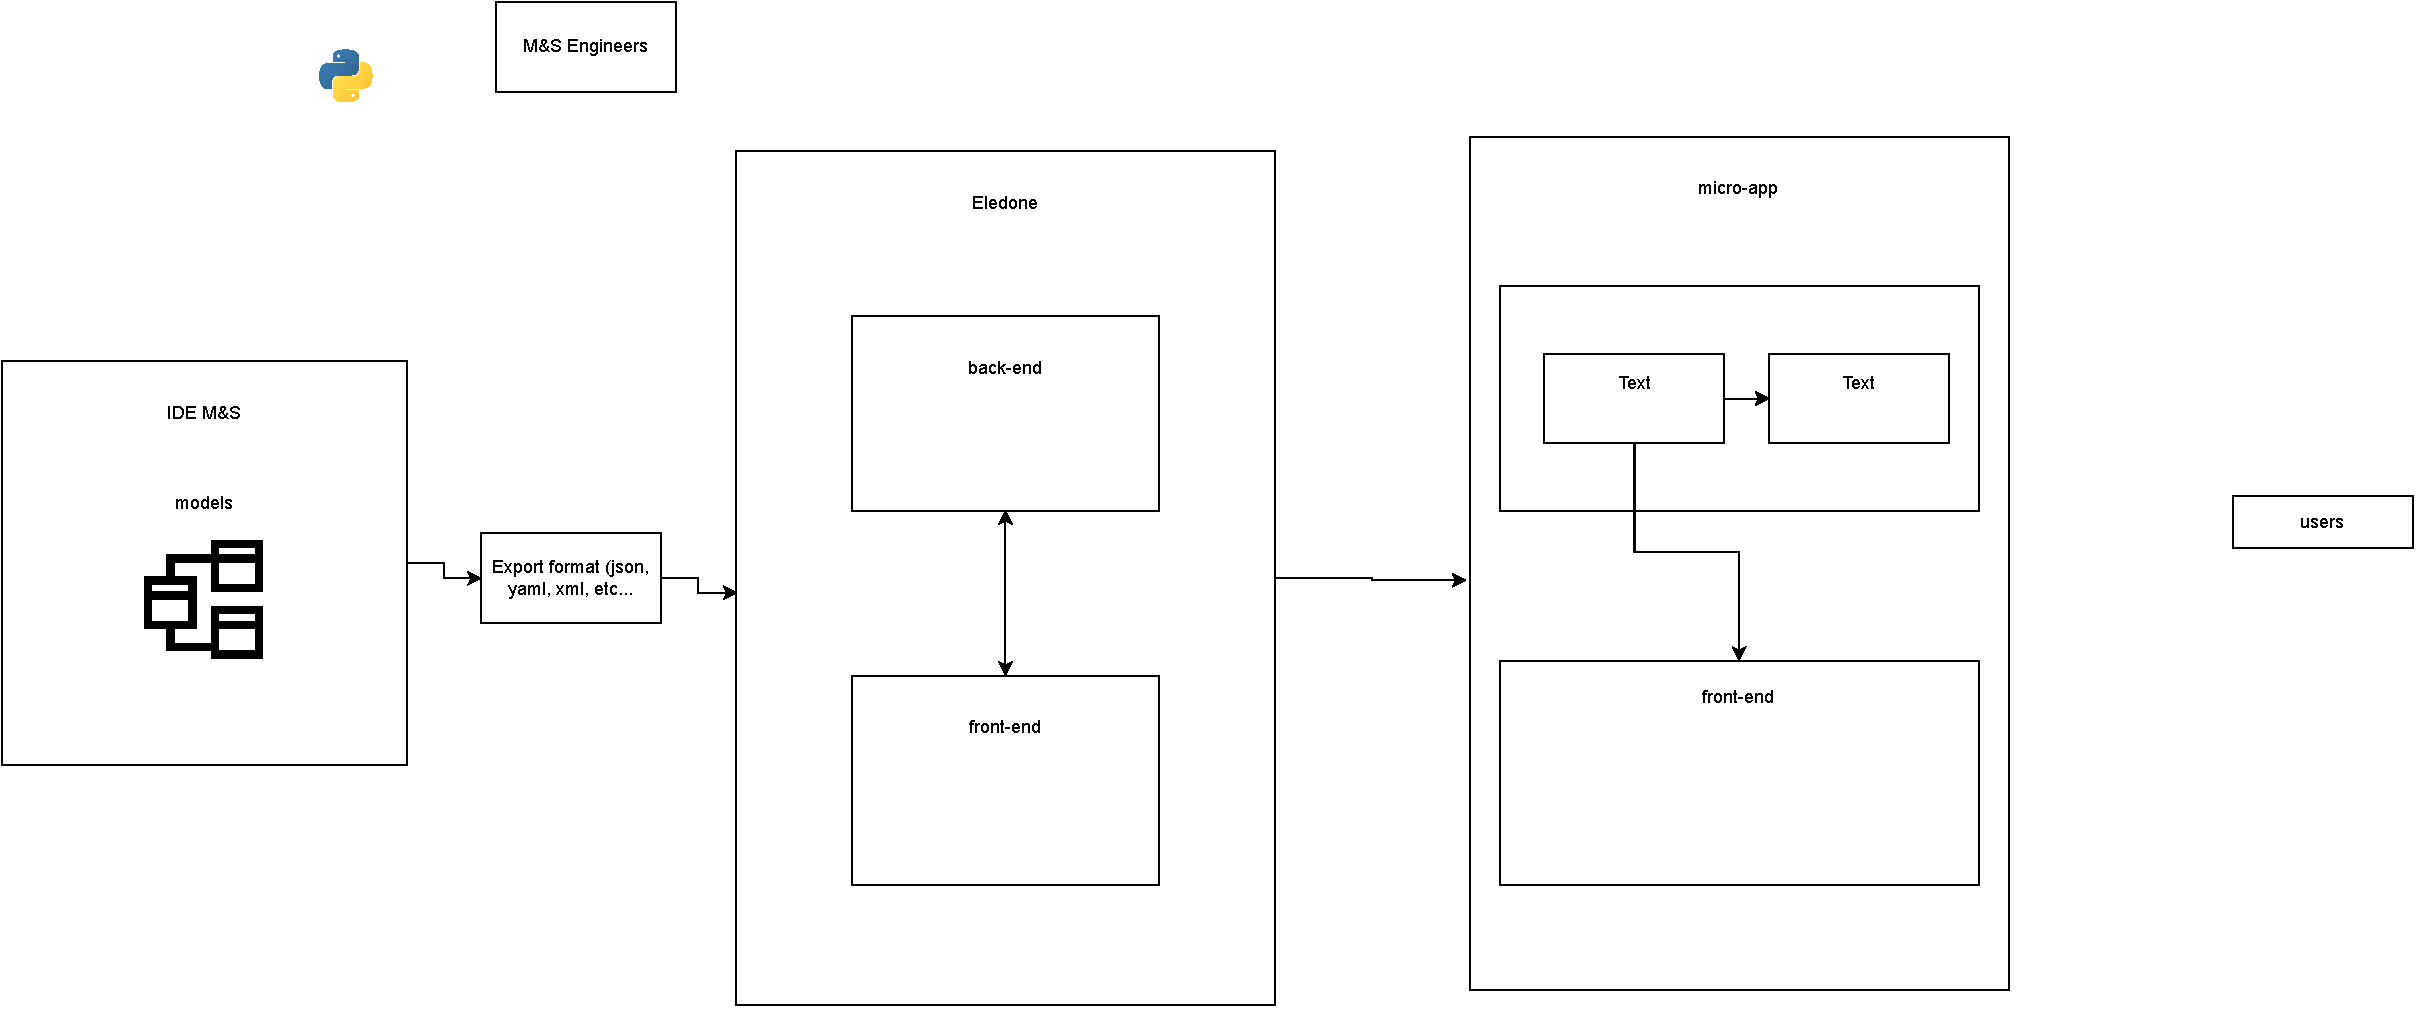
\includegraphics[width=15cm]{figures/architecture_global.pdf}
  \caption{Fonctionnement global du projet}
  \label{fig:fonctionnement-lobal-projet}
\end{figure}

exemple de légende possible
\begin{enumerate}
  \item description 1
  \item description 2
  \item description 3
\end{enumerate}

\chapter{Analyse des composants individuels}

\begin{itemize}[label=$\bullet$]
  \item The first item of the list.
\end{itemize}

\section{L'export d'un modèle de simulation}

\section{L'application Eledone}


\subsection*{Front-end}

\subsection*{Back-end}

\section{Les micro-apps générer par Eledone}

\subsection*{Front-end}

\gls{pdonnées}

\subsection*{Back-end}

% ====================== PARTIE 3  ==========================



\part{Conception}

\begin{itemize}[label=$\bullet$]
  \item Étudier les enjeux lier à la conception et faire le lien avec la partie Analyse
\end{itemize}

\chapter{Conception globale}

\begin{itemize}[label=$\bullet$]
  \item The first item of the list.
\end{itemize}

\chapter{Conception des composants individuels}

\begin{itemize}[label=$\bullet$]
  \item The first item of the list.
\end{itemize}





\cleardoublepage

% ====================== PARTIE 4  ==========================

\part{Le projet après le stage}

\begin{itemize}[label=$\bullet$]
  \item The first item of the list.
\end{itemize}

\chapter{Pistes de réalisation}

\begin{itemize}[label=$\bullet$]
  \item Listé des ressources d'apprentissage lié aux compétences nécessaire eu développement du projet
\end{itemize}

\chapter{Pistes d'évaluation}

\begin{itemize}[label=$\bullet$]
  \item Discuter des possibilités de tests pour chaque élément.
\end{itemize}

\chapter{Projets annexes / améliorations possibles}

\begin{itemize}[label=$\bullet$]
  \item Parler de l'objectif de transformer Eledone en un outil complet de développement et d'export de simulations
  \item envisager les possibilités de faire une version d'Eledone pour l'intelligence artificielle
\end{itemize}

\cleardoublepage

\bookmarksetup{startatroot}

\printbibliography[
  heading=bibintoc,
  title=Bibliographie / Webographie
]

\cleardoublepage


\listoffigures
\cleardoublepage

\listoftables
\cleardoublepage

%%% \newpage just to demonstrate that links are correct
\newpage
\printglossaries

\cleardoublepage
\renewcommand{\thesubsection}{\Roman{subsection}}



\cleardoublepage
\thispagestyle{empty}

\section*{Résumé}
\phantomsection
\addcontentsline{toc}{chapter}{Résumé}



{\bf Mots-clés :}

\end{document}
1